\documentclass{article}
\usepackage[margin=12mm]{geometry}
\usepackage{hyperref}

\usepackage{tikz}

\usepackage[
% school,
% simplified
]{pgf-umlcd}

%%%%%%%%%%%%%%%%%%%%%%%%%%%%%%%%%%%%%%%%%%%%%%%%%%%%%%%%%%%%%%%%%
\usepackage{listings}
\usepackage{color}
\definecolor{listinggray}{gray}{0.92}
\lstset{ %
language=[LaTeX]TeX,
breaklines=true,
frame=single,
% frameround=tttt,
basicstyle=\footnotesize\ttfamily,
backgroundcolor=\color{listinggray},
keywordstyle=\color{blue}
}
%%%%%%%%%%%%%%%%%%%%%%%%%%%%%%%%%%%%%%%%%%%%%%%%%%%%%%%%%%%%%%%%%

%%%%%%%%%%%%%%%%%%%%%%%%%%%%%%%%%%%%%%%%%%%%%%%%%%%%%%%%%%%%%%%%%
\hypersetup{
  colorlinks=true,
  linkcolor=blue,
  anchorcolor=black,
  citecolor=olive,
  filecolor=magenta,
  menucolor=red,
  urlcolor=blue
}
%%%%%%%%%%%%%%%%%%%%%%%%%%%%%%%%%%%%%%%%%%%%%%%%%%%%%%%%%%%%%%%%%

%%%%%%%%%%%%%%%%%%%%%%%%%%%%%%%%%%%%%%%%%%%%%%%%%%%%%%%%%%%%%%%%%
\newcommand{\demo}[2][1]{
\begin{minipage}{.49\linewidth}
\centering
\resizebox{#1\linewidth}{!}{
\input{demo/#2}
}
\end{minipage}
\hspace{0.01\linewidth}
\begin{minipage}{.5\linewidth}
\lstinputlisting{demo/#2}
\end{minipage}
}
%%%%%%%%%%%%%%%%%%%%%%%%%%%%%%%%%%%%%%%%%%%%%%%%%%%%%%%%%%%%%%%%%

%%%%%%%%%%%%%%%%%%%%%%%%%%%%%%%%%%%%%%%%%%%%%%%%%%%%%%%%%%%%%%%%%
\newcommand{\example}[1]{
\resizebox{\linewidth}{!}{
\input{demo/#1}
}
\lstinputlisting{demo/#1}
}
%%%%%%%%%%%%%%%%%%%%%%%%%%%%%%%%%%%%%%%%%%%%%%%%%%%%%%%%%%%%%%%%% 

\renewcommand{\familydefault}{\ttdefault}

\begin{document}

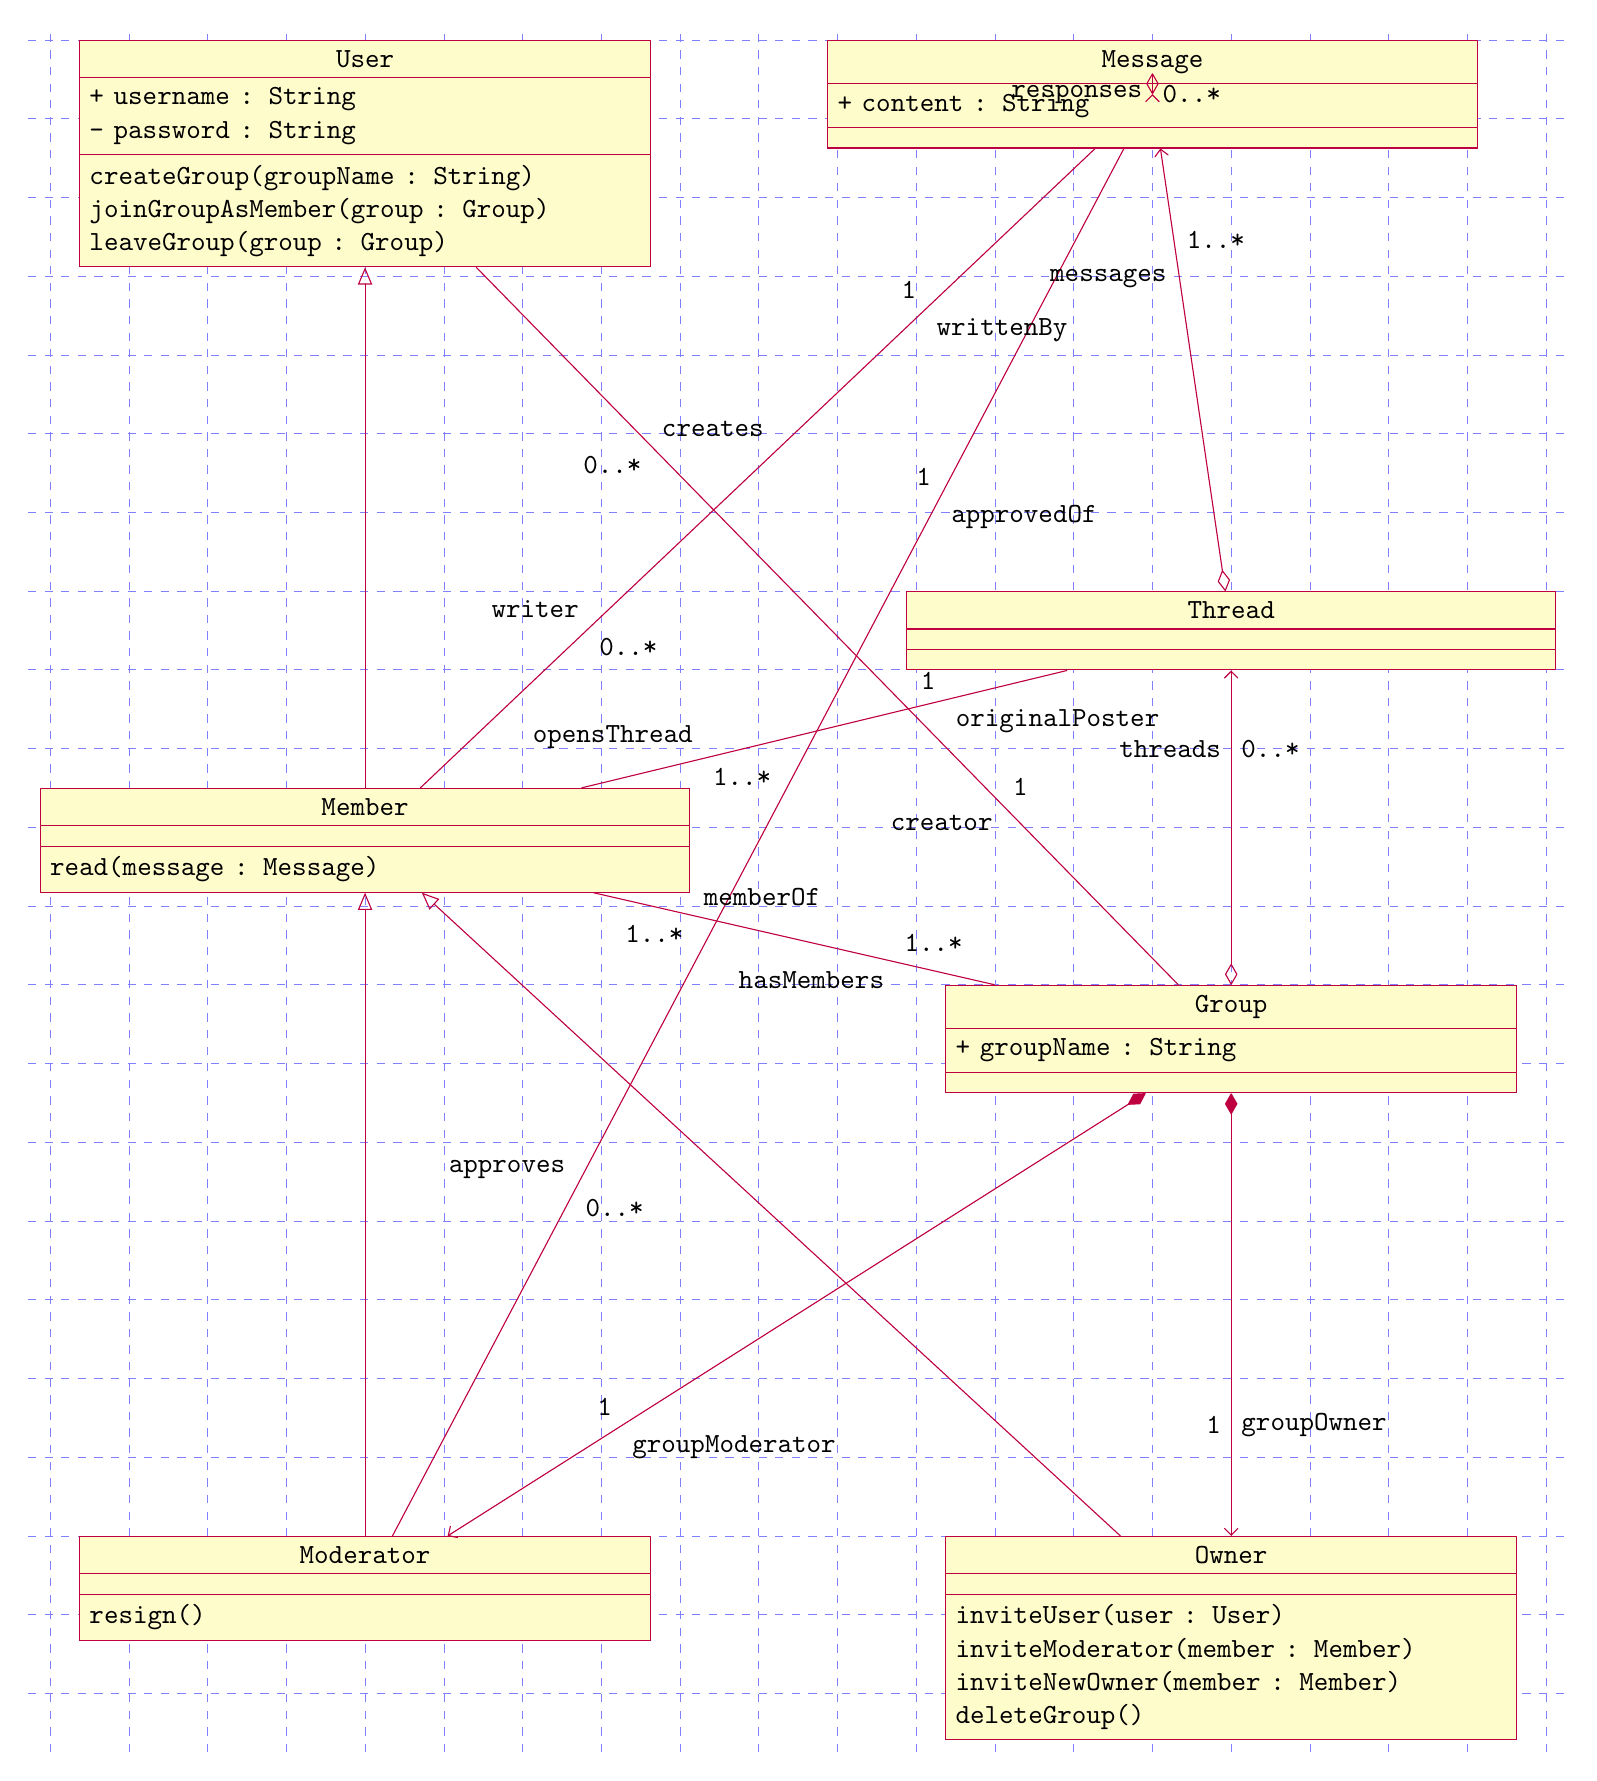
\begin{tikzpicture}[show background grid]

	\begin{class}[text width=7cm]{Group}{11,12}
	
		\attribute{+ groupName : String}
	    
	\end{class}
	
	\begin{class}[text width=7cm]{User}{0,24}
	
		\operation{createGroup(groupName : String)}
		\operation{joinGroupAsMember(group : Group)}
		\operation{leaveGroup(group : Group)}
		
		\attribute{+ username : String}
		\attribute{- password : String}
	    
	\end{class}
	
	\begin{class}[text width=8cm]{Member}{0,14.5}
	
		\inherit{User}
		
		\operation{read(message : Message)}
	    
	\end{class}
	
	\begin{class}[text width=8cm]{Message}{10,24}
	
		\attribute{+ content : String}
	    
	\end{class}
	
	
	\begin{class}[text width=8cm]{Thread}{11,17}
	
		
	    
	\end{class}
	
	\begin{class}[text width=7cm]{Moderator}{0,5}
	
		\inherit{Member}
		
		\operation{resign()}
	    
	\end{class}
	
	\begin{class}[text width=7cm]{Owner}{11,5}
	
		\inherit{Member}
		
		\operation{inviteUser(user : User)}
		\operation{inviteModerator(member : Member)}
		\operation{inviteNewOwner(member : Member)}
		\operation{deleteGroup()}
	    
	\end{class}
	
	\composition{Group}{groupOwner}{1}{Owner}
	\composition{Group}{groupModerator}{1}{Moderator}
	\association{Moderator}{approves}{0..*}{Message}{1}{approvedOf}
	\association{Member}{writer}{0..*}{Message}{1}{writtenBy}
	\association{User}{creates}{0..*}{Group}{1}{creator}
	\association{Member}{memberOf}{1..*}{Group}{1..*}{hasMembers}
	\association{Thread}{originalPoster}{1}{Member}{1..*}{opensThread}
	\aggregation{Thread}{messages}{1..*}{Message}
	\aggregation{Message}{responses}{0..*}{Message}
	\aggregation{Group}{threads}{0..*}{Thread}
	
\end{tikzpicture}


\end{document}